\section{Ejercicio 1: Conexión a datos de Power BI - Tarea 1: Preparar el Medio Ambiente} 

1. Ensure that the MSL-TMG1, 20778A-MIA-DC and 20778A-MIA-SQL virtual machines are running, and then log on to 20778A-MIA-SQL as ADVENTUREWORKS/Student with the password Pa\$\$w0rd. \\
2. In the D:/Labfiles/Lab06/Starter folder, right-click Setup.cmd, and then click Run as administrator. \\
3. In the User Account Control dialog box, click Yes. \\
4. At the command prompt, if prompted, press Y, wait for the script to finish, and then press Enter to close the command window. \\
5. If you do not have a Power BI login, open Internet Explorer, go to https://powerbi.microsoft.com/en-us/documentation/powerbi-admin-signing-up-for-powerbi-with-a-new-office-365-trial, and follow the steps to create an account. \\
6. In Internet Explorer, go to https://www.microsoft.com/enus/download/details.aspx?id=45331, and then click Download. \\
7. On the Choose the download you want page, select the PBIDesktop\_x64.msi check box, and then click Next.\\
8. In the message box, click Run. \\
9. In the Microsoft Power BI Desktop (x64) Setup dialog box, on the Welcome to the Microsoft Power BI Desktop (x64) Setup Wizard page, click Next.\\
10. On the Microsoft Software License Terms page, select the I accept the terms in the License Agreement check box, and then click Next.\\
11. On the Destination Folder page, click Next.\\
12. On the Ready to install Microsoft Power BI Desktop (x64) page, click Install.\\
13. In the User Account Control dialog box, click Yes.\\
14. On the Completed the Microsoft Power BI Desktop (x64) Setup Wizard page, clear the Launch Microsoft Power BI Desktop check box, and then click Finish.\\
15. Close Internet Explorer.\\

	\begin{center}
	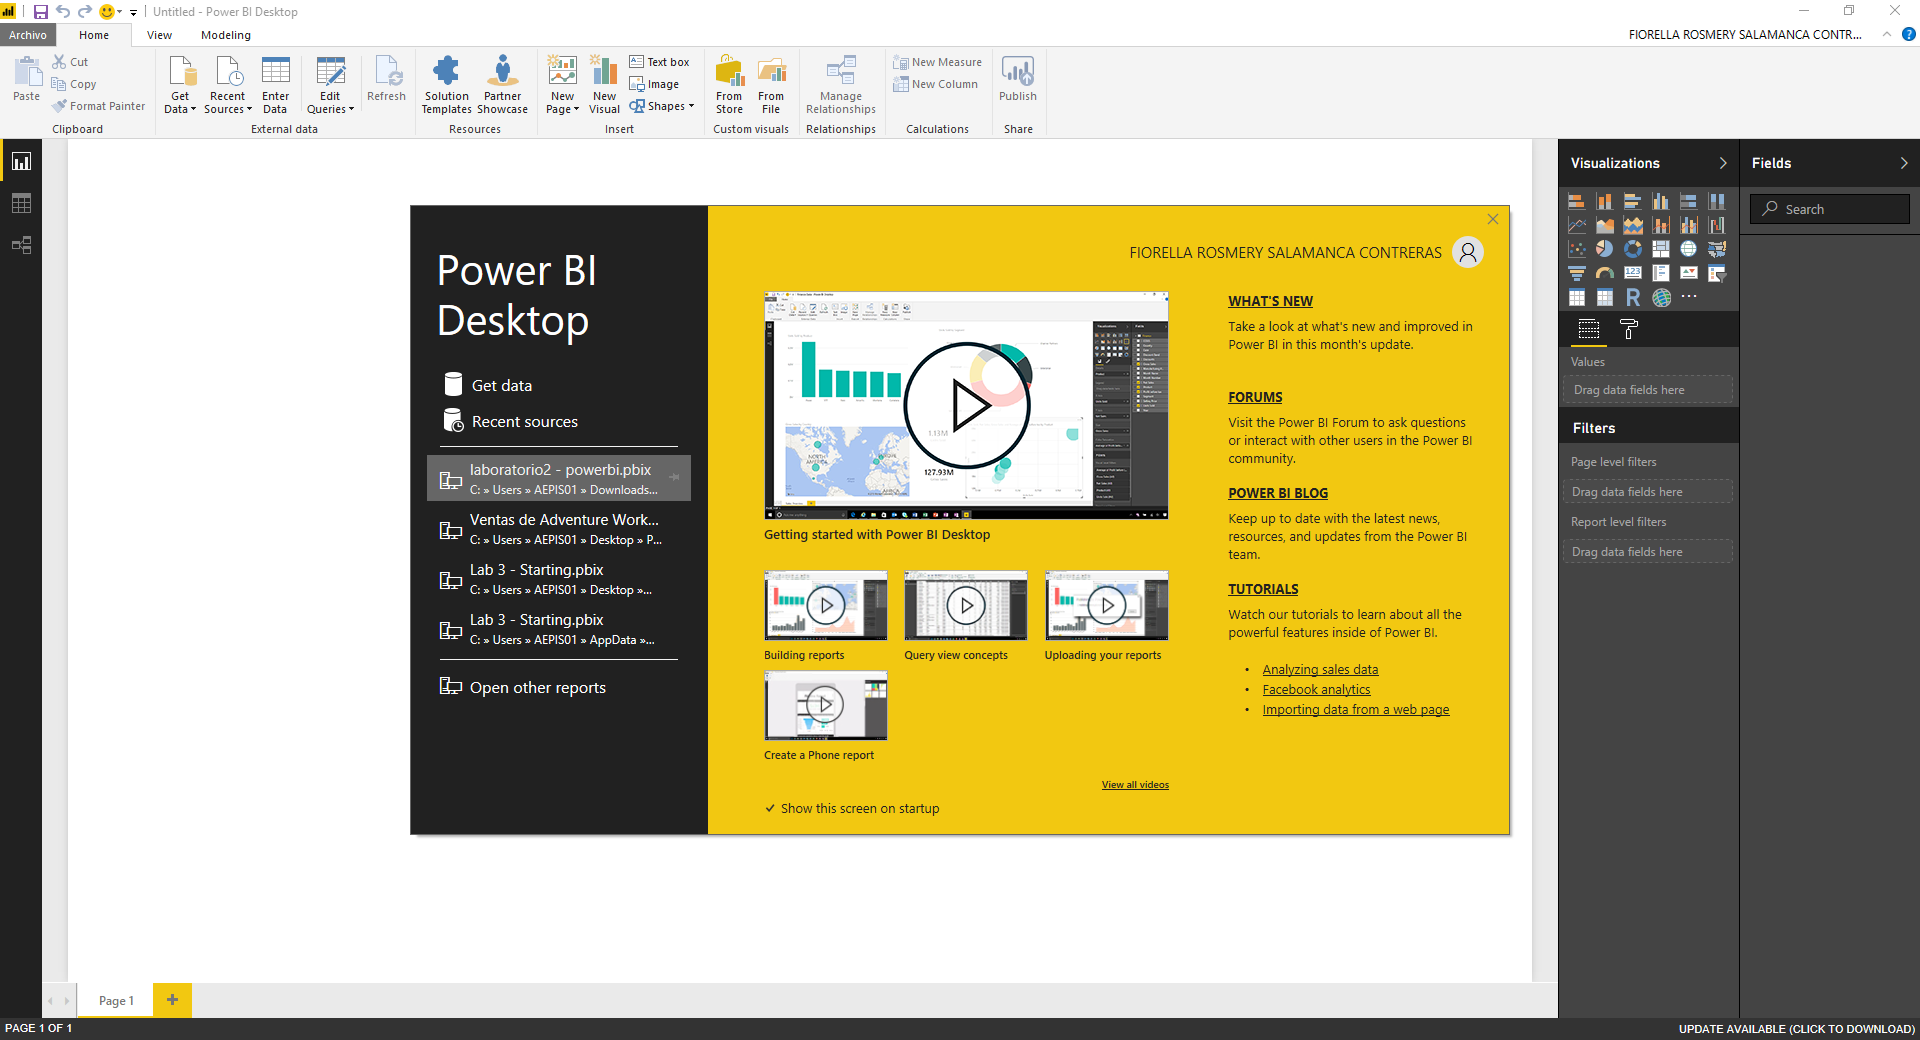
\includegraphics[width=15cm]{./Imagenes/Ejercicio1/Tarea2/3}
	\end{center}	